\documentclass[12pt]{report}

\def\arraystretch{1.2}%

\usepackage{amsmath}
\usepackage{mathtools}
\usepackage{graphicx}
\usepackage{dirtytalk}
\usepackage{float}
\usepackage{xcolor}
\usepackage{todonotes}
\usepackage{parskip}
\usepackage{tabularx}
\usepackage{adjustbox}

\title{Support Vector Machines (SVMs)}
\author{Lavesh Panjwani - K21204134}
\date{2023-03-29}
\setcounter{chapter}{1}

\graphicspath{ {./images/} }

\begin{document}

\maketitle

\tableofcontents

\pagebreak

\chapter{Coursework 2}

\section{Question 1}

\textbf{Q.} Write down the first 7 digits of your student ID as s1s2s3s4s5s6s7.\newline\newline
\textbf{A.} Student Number = 21204134

\section{Question 2}

\textbf{Q.} Find R1 which is the remainder of s1+s2+s3+s4+s5+s6+s7\newline\newline
\textbf{A.} \newline

\[{(2 + 1 + 2 + 0 + 4 + 1 + 3 + 4)} \mod 4 = 1 \]\newline\newline
Since Reminder is \textbf{1}, the method selected is \textbf{One against all}

\section{Question 3}

\textbf{Q.} Create a linearly separable two-dimensional dataset of your own, which consists of
3 classes. List the dataset in the format as shown in Table 2. Each class should
contain at least 10 samples and all three classes have the same number of samples.\newline\newline

\textbf{A.}\newline

\begin{table}[H]
	\centering
	\begin{tabular}{|c | c | c|}
		\hline
		Sample of Class 1 & Sample of Class 2 & Sample of Class 3 \\ [0.5ex]
		\hline\hline
		$x_{1}=$(5,1)     & $x_{11}=$(9,9)    & $x_{21}=$(11,5)   \\
		\hline
		$x_{2}=$(2,5)     & $x_{12}=$(7,8)    & $x_{22}=$(10,2)   \\
		\hline
		$x_{3}=$(4,4)     & $x_{13}=$(5,9)    & $x_{23}=$(11,3)   \\
		\hline
		$x_{4}=$(2,3)     & $x_{14}=$(9,15)   & $x_{24}=$(12,5)   \\
		\hline
		$x_{5}=$(3,1)     & $x_{15}=$(7,11)   & $x_{25}=$ (18,1)  \\
		\hline
		$x_{6}=$(4,2)     & $x_{16}=$(8,15)   & $x_{26}=$(16,4)   \\
		\hline
		$x_{7}=$(3,3)     & $x_{17}=$(7,13)   & $x_{27}=$(14,4)   \\
		\hline
		$x_{8}=$(2,2)     & $x_{18}=$(8,14)   & $x_{28}=$(12,4)   \\
		\hline
		$x_{9}=$(3,4)     & $x_{19}=$(6,14)   & $x_{29}=$(17,5)   \\
		\hline
		$x_{10}=$(4,3)    & $x_{20}=$(10,14)  & $x_{30}=$(13,5)   \\
		\hline
	\end{tabular}
	\caption{Classes Sample}
\end{table}

\section{Question 4}

\textbf{Q.} Plot the dataset in Q3 to show that the samples are linearly separable. Explain
why your dataset is linearly separable. Hint: the Matlab built-in function
plot can be used and show some example hyperplanes which can linearly separable
the datasets. Identify which hyperplane is for which classes.\newline\newline
\textbf{A.}

\begin{figure}[H]
	\centering
	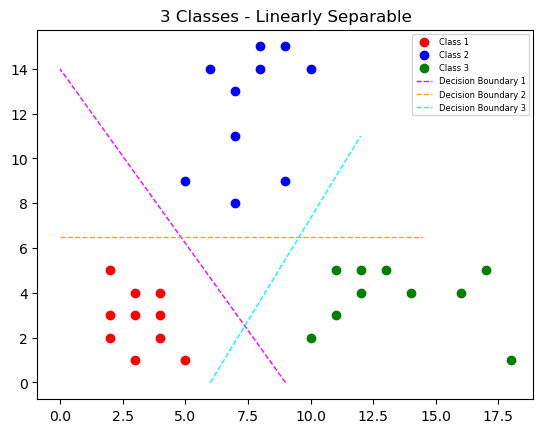
\includegraphics[width=\textwidth]{plot.png}
	\caption{Plotted Dataset}
\end{figure}

Datasets are linearly separable when it is possible to separate the data points of different classes using a straight line or a hyperplane in the feature space. If there exists a boundary or decision boundary that separates the different classes of the dataset, such that all points of one class are on one side of the boundary and all points of the other class are on the other side of the boundary, then the dataset is linearly separable.

\section{Question 5}

\textbf{Q.} According to the method obtained in Q2, draw a block diagram at SVM level to
show the structure of the multi-class classifier constructed by linear SVMs. Explain
the design (e.g., number of inputs, number of outputs, number of SVMs used, class
label assignment, etc.) and describe how this multi-class classifier works.\newline\newline
\textbf{A.} In this approach, the classifier is trained to distinguish one class from all the others. This is done by training a separate SVM classifier for each class, where the positive class is the one being considered and the negative classes are all the other classes combined.
To classify a new data point, the classifier applies all the trained binary classifiers to the point and assigns the class that the majority votes.\newline\newline

\begin{figure}[H]
	\centering
	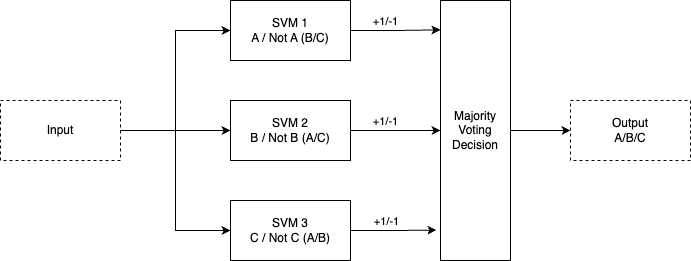
\includegraphics[width=\textwidth]{block.png}
	\caption{Block Diagram of Designed SVM}
\end{figure}

Number of classifiers = \textit{\textbf{R}} 2-class classifiers are needed to classify \textit{\textbf{R}} classes.
In this case, considering we have 3 classes, we need to have \textit{\textbf{R}} = 3 Classifiers.

\begin{table}[H]
	\centering
	\begin{tabular}{|c | c|}
		\hline
		SVM Number & Description                           \\ [0.5ex]
		\hline
		SVM 1      & Class 1 against (Class 2 and Class 3) \\
		\hline
		SVM 2      & Class 2 against (Class 1 and Class 3) \\
		\hline
		SVM 3      & Class 3 against (Class 1 and Class 2) \\
		\hline
	\end{tabular}
	\caption{SVM Description}
\end{table}



\textbf{Design Statistics:}\newline\newline
Number of Inputs = 2 (x, y coordinates)\newline
Number of Outputs = 3 (Either Class A, B, C)\newline
Number of SVMs Used = 3\newline
Decision Methodology  = Choosing the class with majority votes\newline\newline

\textbf{Learning of the SVM:}\newline

The SVMs are trained using the training data. The training data is the same as the data used to plot the graph in Question 4.

A 2-class SVM is trained to distinguish between the positive class and the negative class. The positive class is the class that is being considered and the negative class is the combination of all the other classes. The SVM is trained to output +1 for the positive class and -1 for the negative class.

Classifiers are trained for $C_{r}$ against $C_{1} \cup C_{2} \cup \cdots \cup C_{r-1} \cup C_{r+1} \cup \cdots \cup C_{n}$. The positive class is $C_{r}$ and the negative class is $C_{1} \cup C_{2} \cup \cdots \cup C_{r-1} \cup C_{r+1} \cup \cdots \cup C_{n}$.

Classifiers use the formula $w_{i}^{i}x + w_{0}^{i}$ to classify the data points. The data points are classified as belonging to the positive class if the output is greater than 0 and as belonging to the negative class if the output is less than 0.

\vspace*{10pt}

\textbf{Decision Making of the SVM:}\newline

Let's work through an example with this system:\newline

\textbf{Step 1}: Find the outputs of the SVMs:

\begin{table}[H]
	\centering
	\begin{tabular}{|c | c|}
		\hline
		SVM Number & Output                      \\ [0.5ex]
		\hline
		SVM 1      & A / Class 1 (+1)            \\
		\hline
		SVM 2      & NOT B / (Class 1 or 3) (-1) \\
		\hline
		SVM 3      & NOT C / (Class 1 or 2) (-1) \\
		\hline
	\end{tabular}
	\caption{Example SVM Output}
\end{table}

\textbf{Step 2}: Compute the number of votes each class has

\begin{equation*}
	\begin{aligned}
		\textbf{Class 1} & = Vote_{S1} + Vote_{S2} +  Vote_{S3} \\
		                 & = 3
	\end{aligned}
\end{equation*}

\begin{equation*}
	\begin{aligned}
		\textbf{Class 2} & =  Vote_{S3} \\
		                 & = 1
	\end{aligned}
\end{equation*}

\begin{equation*}
	\begin{aligned}
		\textbf{Class 3} & =  Vote_{S2} \\
		                 & = 1
	\end{aligned}
\end{equation*}\newline


\textbf{Step 3}: Pick which class has the majority of the votes

\vspace{10pt}

Given that \textbf{Class 1} has \textbf{3} votes is the winner.

\vspace{10pt}

\textbf{Caveats:}\newline


\begin{enumerate}
	\item One
	      Some regions cannot be classified using Hard SVM classifiers. Instead using a Soft SVM classifier can classify all regions. Using a Soft SVM classifier can misclassify regions around the boundaries.
\end{enumerate}

\section{Question 6}

\begin{figure}[H]
	\centering
	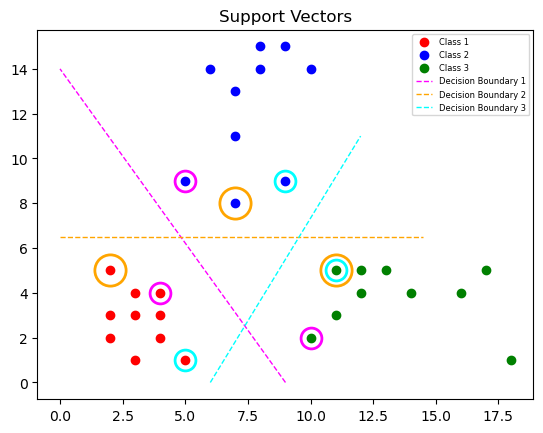
\includegraphics[width=\textwidth]{supportvectors.png}
	\caption{Support Vectors of Hyperplanes}
	Colored in Hyperlane Colours
\end{figure}

\pagebreak

\subsection{Hyperlane / Decision Boundary 1 (Magenta):}

Class 1 (+1):
\begin{equation*}
	\begin{aligned}
		x_{3} = \begin{bmatrix}
			        4 \\
			        4
		        \end{bmatrix}
	\end{aligned}
\end{equation*}

Class 2 (-1):
\begin{equation*}
	\begin{aligned}
		x_{22} = \begin{bmatrix}
			         10 \\
			         2
		         \end{bmatrix}
		x_{13} = \begin{bmatrix}
			         5 \\
			         9
		         \end{bmatrix}
	\end{aligned}
\end{equation*}

Here:\newline
\textbf{Class 1} is labeled as +1 \newline
\textbf{Class 2} is labeled as -1

\textbf{Step 1:}

From the Lectures Slides, we know that the $w$ is defined by the following equation:

\begin{equation*}
	\begin{aligned}
		w & = \lambda_{3}y_{3}X_{3} + \lambda_{22}y_{22}X_{22} + \lambda_{13}y_{13}X_{13}                                   \\
		  & = (\lambda_{3} * 1 * \begin{bmatrix}
			                         4 \\
			                         4
		                         \end{bmatrix}) + (\lambda_{22} * -1 * \begin{bmatrix}
			                                                               10 \\
			                                                               2
		                                                               \end{bmatrix}) + (\lambda_{13} * -1 * \begin{bmatrix}
			                                                                                                     5 \\
			                                                                                                     9
		                                                                                                     \end{bmatrix})
	\end{aligned}
\end{equation*}

\vspace{20pt}
\textbf{Step 2:}

\begin{equation*}
	\begin{aligned}
		y_{3} & =  w^T x_{3} + w_{0} = 1            \\
		      & = \begin{pmatrix}
			          \begin{pmatrix}
				\lambda_{3}\begin{bmatrix}
					           4 \\
					           4
				           \end{bmatrix} -

				\lambda_{22}\begin{bmatrix}
					            10 \\
					            2
				            \end{bmatrix}
				-

				\lambda_{13}\begin{bmatrix}
					            5 \\
					            9
				            \end{bmatrix}
			\end{pmatrix}  ^ T
			          \begin{bmatrix}
				4 \\
				4
			\end{bmatrix} + w_{0}
		          \end{pmatrix} = 1
	\end{aligned}
\end{equation*}

\begin{equation*}
	\begin{aligned}
		y_{22} & =  w^T x_{22} + w_{0} = -1          \\
		       & = \begin{pmatrix}
			           \begin{pmatrix}
				\lambda_{3}\begin{bmatrix}
					           4 \\
					           4
				           \end{bmatrix} -

				\lambda_{22}\begin{bmatrix}
					            10 \\
					            2
				            \end{bmatrix}
				-

				\lambda_{13}\begin{bmatrix}
					            5 \\
					            9
				            \end{bmatrix}\end{pmatrix}  ^ T
			           \begin{bmatrix}
				10 \\
				2
			\end{bmatrix} + w_{0}
		           \end{pmatrix} = -1
	\end{aligned}
\end{equation*}

\begin{equation*}
	\begin{aligned}
		y_{13} & =  w^T x_{13} + w_{0} = -1          \\
		       & = \begin{pmatrix}
			           \begin{pmatrix}
				\lambda_{3}\begin{bmatrix}
					           4 \\
					           4
				           \end{bmatrix} -

				\lambda_{22}\begin{bmatrix}
					            10 \\
					            2
				            \end{bmatrix}
				-

				\lambda_{13}\begin{bmatrix}
					            5 \\
					            9
				            \end{bmatrix}\end{pmatrix}  ^ T
			           \begin{bmatrix}
				5 \\
				9
			\end{bmatrix} + w_{0}
		           \end{pmatrix} = -1
	\end{aligned}
\end{equation*}

\textbf{Step 3:}
\begin{equation*}
	Solving for \lambda_{3}, \lambda_{22}, \lambda_{13}, w_{0}
\end{equation*}


\begin{equation*}
	\begin{aligned}
		\lambda_{3}\begin{pmatrix}4 \\ 4\end{pmatrix}-\lambda_{22}\begin{pmatrix}10\\ 2\end{pmatrix}-\lambda_{13}\begin{pmatrix}5\\ 9\end{pmatrix}=\begin{pmatrix}4\lambda_{3}-10\lambda_{22}-5\lambda_{13}\\ 4\lambda_{3}-2\lambda_{22}-9\lambda_{13}\end{pmatrix}
	\end{aligned}
\end{equation*}

\begin{equation}
	\begin{aligned}
		\begin{pmatrix}4\lambda_{3}-10\lambda_{22}-5\lambda_{13} & 4\lambda_{3}-2\lambda_{22}-9\lambda_{13}\end{pmatrix}\begin{pmatrix}4 \\ 4\end{pmatrix}=\begin{pmatrix}32\lambda_{3}-48\lambda_{22}-56\lambda_{13}\end{pmatrix}
	\end{aligned}
\end{equation}

\begin{equation}
	\begin{aligned}
		\begin{pmatrix}4\lambda_{3}-10\lambda_{22}-5\lambda_{13} & 4\lambda_{3}-2\lambda_{22}-9\lambda_{13}\end{pmatrix}\begin{pmatrix}10 \\ 2\end{pmatrix}=\begin{pmatrix}48\lambda_{3}-104\lambda_{22}-68\lambda_{13}\end{pmatrix}
	\end{aligned}
\end{equation}

\begin{equation}
	\begin{aligned}             \begin{pmatrix}4\lambda_{3}-10\lambda_{22}-5\lambda_{13}&4\lambda_{3}-2\lambda_{22}-9\lambda_{13}\end{pmatrix}\begin{pmatrix}5\\ 9\end{pmatrix}=\begin{pmatrix}56\lambda_{3}-68\lambda_{22}-106\lambda_{13}\end{pmatrix}
	\end{aligned}
\end{equation}

\begin{equation}
	\lambda_{3}-\lambda_{22}-\lambda_{13}
\end{equation}

Adding the above equations in matrix form:

\begin{equation*}
	\begin{aligned}
		\begin{pmatrix}32 & -48 & -56 & 1 \\ 48&-104&-68&1\\ 56&-68&-106&1\\ 1&-1&-1&0\end{pmatrix}\begin{pmatrix}\lambda_{3}\\ \lambda_{22}\\ \lambda_{13}\\ w_{0}\end{pmatrix}=\begin{pmatrix}1\\ -1\\ -1\\ 0\end{pmatrix}
	\end{aligned}
\end{equation*}

\begin{equation*}
	\begin{aligned}
		\lambda_{3}=\frac{361}{2500},\:\lambda_{22}=\frac{117}{2000},\:\lambda_{13}=\frac{859}{1000},\:w_{0}=\frac{3997}{1000}
	\end{aligned}
\end{equation*}

\vspace{20pt}
\textbf{Step 4:} Solving for $w$

\begin{equation}
	\begin{aligned}
		w & = \lambda_{3}y_{3}X_{3} - \lambda_{22}y_{22}X_{22} - \lambda_{13}y_{13}X_{13}                                                                                                                  \\
		  & = \frac{361}{2500}\begin{pmatrix}4                                      \\ 4\end{pmatrix}-\frac{117}{2000}\begin{pmatrix}10\\ 2\end{pmatrix}-\frac{859}{1000}\begin{pmatrix}5\\ 9\end{pmatrix} \\
		  & = \begin{pmatrix}-\frac{877}{2000}                                      \\ -\frac{3141}{10000}\end{pmatrix}
	\end{aligned}
\end{equation}


\vspace{20pt}

\textbf{Step 5:} Finding Hyperlane Equation

\begin{equation}
	\begin{aligned}
		y & = w^Tx + w_{0} = 0                                                                                                                      \\
		  & = w^T\begin{pmatrix}x_{i}              \\x_{j}\end{pmatrix} + w_{0} = 0                                                                 \\
		  & = \begin{pmatrix}-\frac{877}{2000}     \\ -\frac{3141}{10000}\end{pmatrix}\begin{pmatrix}x_{i}\\x_{j}\end{pmatrix} + \frac{318}{25} = 0 \\
		  & = -\frac{349}{250}\begin{pmatrix}x_{i} \\x_{j}\end{pmatrix} + \frac{318}{25}
	\end{aligned}
\end{equation}


\vspace{20pt}

\pagebreak
\subsection{Hyperlane / Decision Boundary 2 (Orange):}
Class 1 (+1):
\begin{equation*}
	\begin{aligned}
		x_{12} = \begin{bmatrix}
			         7 \\
			         8
		         \end{bmatrix}
	\end{aligned}
\end{equation*}

Class 2 (-1):
\begin{equation*}
	\begin{aligned}
		x_{2} = \begin{bmatrix}
			        2 \\
			        5
		        \end{bmatrix}
		x_{21} = \begin{bmatrix}
			         11 \\
			         5
		         \end{bmatrix}
	\end{aligned}
\end{equation*}

Here:\newline
\textbf{Class 1} is labeled as +1 \newline
\textbf{Class 2} is labeled as -1


\textbf{Step 1:}

\begin{equation*}
	\begin{aligned}
		w & = \lambda_{12}y_{12}X_{12} + \lambda_{2}y_{2}X_{2}   + \lambda_{21}y_{21}X_{21}                                  \\
		  & = (\lambda_{12} * 1 * \begin{bmatrix}
			                          7 \\
			                          8
		                          \end{bmatrix}) + (\lambda_{2} * -1 * \begin{bmatrix}
			                                                               2 \\
			                                                               5
		                                                               \end{bmatrix})  + (\lambda_{21} * -1 * \begin{bmatrix}
			                                                                                                      11 \\
			                                                                                                      5
		                                                                                                      \end{bmatrix})
	\end{aligned}
\end{equation*}

\vspace{20pt}

\textbf{Step 2:}

\begin{equation*}
	\begin{aligned}
		y_{12} & =  w^T x_{12} + w_{0} = 1               \\
		       & = 1 * \begin{pmatrix}
			               \begin{pmatrix}
				\lambda_{12}\begin{bmatrix}
					            7 \\
					            8
				            \end{bmatrix} -

				\lambda_{2}\begin{bmatrix}
					           2 \\
					           5
				           \end{bmatrix} -

				\lambda_{21}\begin{bmatrix}
					            11 \\
					            5
				            \end{bmatrix}
			\end{pmatrix}   ^ T
			               \begin{bmatrix}
				7 \\
				8
			\end{bmatrix} + w_{0}
		               \end{pmatrix} = 1
	\end{aligned}
\end{equation*}

\begin{equation*}
	\begin{aligned}
		y_{2} & =  w^T x_{2} + w_{0} = -1               \\
		      & = 1 * \begin{pmatrix}
			              \begin{pmatrix}
				\lambda_{12}\begin{bmatrix}
					            7 \\
					            8
				            \end{bmatrix} -

				\lambda_{2}\begin{bmatrix}
					           2 \\
					           5
				           \end{bmatrix} -

				\lambda_{21}\begin{bmatrix}
					            11 \\
					            5
				            \end{bmatrix}
			\end{pmatrix}  ^ T
			              \begin{bmatrix}
				2 \\
				5
			\end{bmatrix} + w_{0}
		              \end{pmatrix} = -1
	\end{aligned}
\end{equation*}

\begin{equation*}
	\begin{aligned}
		y_{21} & =  w^T x_{21} + w_{0} = -1              \\
		       & = 1 * \begin{pmatrix}
			               \begin{pmatrix}
				\lambda_{12}\begin{bmatrix}
					            7 \\
					            8
				            \end{bmatrix} -

				\lambda_{2}\begin{bmatrix}
					           2 \\
					           5
				           \end{bmatrix} -

				\lambda_{21}\begin{bmatrix}
					            11 \\
					            5
				            \end{bmatrix}
			\end{pmatrix}  ^ T
			               \begin{bmatrix}
				11 \\
				5
			\end{bmatrix} + w_{0}
		               \end{pmatrix} = -1
	\end{aligned}
\end{equation*}

\textbf{Step 3:}
\begin{equation*}
	Solving for \lambda_{12}, \lambda_{2}, \lambda_{21}, w_{0}
\end{equation*}


\begin{equation*}
	\begin{aligned}
		\lambda_{12}\begin{pmatrix}7 \\ 8\end{pmatrix}-\lambda_{2}\begin{pmatrix}2\\ 5\end{pmatrix}-\lambda_{21}\begin{pmatrix}11\\ 5\end{pmatrix}=\begin{pmatrix}7\lambda_{12}-2\lambda_{2}-11\lambda_{21}\\ 8\lambda_{1}-5\lambda_{2}-5\lambda_{3}\end{pmatrix}
	\end{aligned}
\end{equation*}

\begin{equation}
	\begin{aligned}
		\begin{pmatrix}7\lambda_{12}-2\lambda_{2}-11\lambda_{21} & 8\lambda_{13}-5\lambda_{2}-5\lambda_{21}\end{pmatrix}\begin{pmatrix}7 \\ 8\end{pmatrix}=\begin{pmatrix}113\lambda_{12}-54\lambda_{2}-117\lambda_{21}\end{pmatrix}
	\end{aligned}
\end{equation}

\begin{equation}
	\begin{aligned}
		\begin{pmatrix}7\lambda_{12}-2\lambda_{2}-11\lambda_{21} & 8\lambda_{12}-5\lambda_{2}-5\lambda_{21}\end{pmatrix}\begin{pmatrix}2 \\ 5\end{pmatrix}=\begin{pmatrix}54\lambda_{12}-29\lambda_{2}-47\lambda_{21}\end{pmatrix}
	\end{aligned}
\end{equation}

\begin{equation}
	\begin{aligned}
		\begin{pmatrix}7\lambda_{12}-2\lambda_{2}-11\lambda_{21} & 8\lambda_{12}-5\lambda_{2}-5\lambda_{21}\end{pmatrix}\begin{pmatrix}5 \\ 9\end{pmatrix}=\begin{pmatrix}117\lambda_{12}-47\lambda_{2}-146\lambda_{21}\end{pmatrix}
	\end{aligned}
\end{equation}

\begin{equation}
	\begin{aligned}
		\begin{pmatrix}\lambda_{1}-\lambda_{2}-\lambda_{21}\end{pmatrix}
	\end{aligned}
\end{equation}


Adding the above equations in matrix form:

\begin{equation*}
	\begin{aligned}
		\begin{pmatrix}113 & -54 & -117 & 1 \\ \:54&-29&-47&1\\ \:117&-47&-146&1\\ \:1&-1&-1&0\end{pmatrix}\begin{pmatrix}\lambda_{12}\\ \lambda_{2}\\ \lambda_{21}\\ w_{0}\end{pmatrix}=\begin{pmatrix}1\\ -1\\ -1\\ 0\end{pmatrix}
	\end{aligned}
\end{equation*}

\begin{equation*}
	\begin{aligned}
		\lambda_{12}=\frac{2}{9},\:\lambda_{2}=\frac{8}{81},\:\lambda_{21}=\frac{10}{81},\:w_{0}=-\frac{13}{3}
	\end{aligned}
\end{equation*}

\vspace{20pt}
\textbf{Step 4:} Solving for $w$

\begin{equation}
	\begin{aligned}
		w & = \lambda_{12}y_{1}X_{12} - \lambda_{2}y_{2}X_{2} - \lambda_{21}y_{21}X_{21}                                                                                                            \\
		  & = \frac{2}{9}\begin{pmatrix}7                                           \\ 8\end{pmatrix}-\frac{8}{81}\begin{pmatrix}2\\ 5\end{pmatrix}-\frac{10}{81}\begin{pmatrix}11\\ 5\end{pmatrix} \\
		  & = \begin{pmatrix}0                                                      \\ \frac{2}{3}\end{pmatrix}
	\end{aligned}
\end{equation}

\vspace{20pt}
\textbf{Step 5:} Finding Hyperlane Equation

\begin{equation}
	\begin{aligned}
		y & = w^Tx + w_{0} = 0                                                                                            \\
		  & = w^T\begin{pmatrix}x_{i} \\x_{j}\end{pmatrix} + w_{0} = 0                                                    \\
		  & = \begin{pmatrix}0        \\ \frac{2}{3}\end{pmatrix}\begin{pmatrix}x_{i}\\x_{j}\end{pmatrix}+-\frac{13}{3}=0 \\
		  & = 6.5
	\end{aligned}
\end{equation}

\pagebreak
\subsection{Hyperlane / Decision Boundary 3 (Cyan):}

Class 1 (+1):
\begin{equation*}
	\begin{aligned}
		x_{21} = \begin{bmatrix}
			         11 \\
			         5
		         \end{bmatrix}
	\end{aligned}
\end{equation*}

Class 2 (-1):
\begin{equation*}
	\begin{aligned}
		x_{1} = \begin{bmatrix}
			        5 \\
			        1
		        \end{bmatrix}
		x_{11} = \begin{bmatrix}
			         9 \\
			         9
		         \end{bmatrix}
	\end{aligned}
\end{equation*}

Here:\newline
\textbf{Class 1} is labeled as +1 \newline
\textbf{Class 2} is labeled as -1

\textbf{Step 1:}\newline\newline
\begin{equation*}
	\begin{aligned}
		w & = \lambda_{21}y_{21}x_{21} + \lambda_{1}y_{1}X_{1} + \lambda_{11}y_{11}X_{11}                                  \\
		  & = (\lambda_{21} * 1 * \begin{bmatrix}
			                          11 \\
			                          5
		                          \end{bmatrix}) + (\lambda_{1} * 1 * \begin{bmatrix}
			                                                              5 \\
			                                                              1
		                                                              \end{bmatrix}) + (\lambda_{11} * -1 * \begin{bmatrix}
			                                                                                                    9 \\
			                                                                                                    9
		                                                                                                    \end{bmatrix})
	\end{aligned}
\end{equation*}

\textbf{Step 2:}

\begin{equation*}
	\begin{aligned}
		y_{1} & =  w^T x_{21} + w_{0} = 1            \\
		      & = \begin{pmatrix}
			          \begin{pmatrix}
				\lambda_{21}\begin{bmatrix}
					            11 \\
					            5
				            \end{bmatrix} -

				\lambda_{1}\begin{bmatrix}
					           5 \\
					           1
				           \end{bmatrix} -

				\lambda_{11}\begin{bmatrix}
					            9 \\
					            9
				            \end{bmatrix}
			\end{pmatrix}  ^ T
			          \begin{bmatrix}
				11 \\
				5
			\end{bmatrix} + w_{0}
		          \end{pmatrix} = 1
	\end{aligned}
\end{equation*}

\begin{equation*}
	\begin{aligned}
		y_{21} & =  w^T x_{1} + w_{0} = 1             \\
		       & = \begin{pmatrix}
			           \begin{pmatrix}
				\lambda_{21}\begin{bmatrix}
					            11 \\
					            5
				            \end{bmatrix} -

				\lambda_{1}\begin{bmatrix}
					           5 \\
					           1
				           \end{bmatrix} -

				\lambda_{11}\begin{bmatrix}
					            9 \\
					            9
				            \end{bmatrix}
			\end{pmatrix}  ^ T
			           \begin{bmatrix}
				5 \\
				1
			\end{bmatrix} + w_{0}
		           \end{pmatrix} = -1
	\end{aligned}
\end{equation*}

\begin{equation*}
	\begin{aligned}
		y_{11} & =  w^T x_{11} + w_{0} = -1           \\
		       & = \begin{pmatrix}
			           \begin{pmatrix}
				\lambda_{21}\begin{bmatrix}
					            11 \\
					            5
				            \end{bmatrix} -

				\lambda_{1}\begin{bmatrix}
					           5 \\
					           1
				           \end{bmatrix} -

				\lambda_{11}\begin{bmatrix}
					            9 \\
					            9
				            \end{bmatrix}
			\end{pmatrix}  ^ T
			           \begin{bmatrix}
				9 \\
				9
			\end{bmatrix} + w_{0}
		           \end{pmatrix} = -1
	\end{aligned}
\end{equation*}

\vspace{20pt}

\textbf{Step 3:}
\begin{equation*}
	Solving for \lambda_{21}, \lambda_{1}, \lambda_{11}, w_{0}
\end{equation*}


\begin{equation*}
	\begin{aligned}
		\lambda_{21}\begin{pmatrix}11 \\ 5\end{pmatrix}-\lambda_{1}\begin{pmatrix}5\\ 1\end{pmatrix}-\lambda_{11}\begin{pmatrix}9\\ 9\end{pmatrix}=\begin{pmatrix}11\lambda_{21}-5\lambda_{1}-9\lambda_{11}\\ 5\lambda_{21}-\lambda_{1}-9\lambda_{11}\end{pmatrix}
	\end{aligned}
\end{equation*}

\begin{equation}
	\begin{aligned}
		\begin{pmatrix}11\lambda_{21}-5\lambda_{1}-9\lambda_{11} & 5\lambda_{21}-\lambda_{1}-9\lambda_{11}\end{pmatrix}\begin{pmatrix}11 \\ 5\end{pmatrix}=\begin{pmatrix}146\lambda_{21}-60\lambda_{1}-144\lambda_{11}\end{pmatrix}
	\end{aligned}
\end{equation}

\begin{equation}
	\begin{aligned}
		\begin{pmatrix}11\lambda_{21}-5\lambda_{1}-9\lambda_{11} & 5\lambda_{21}-\lambda_{1}-9\lambda_{11}\end{pmatrix}\begin{pmatrix}5 \\ 1\end{pmatrix}=\begin{pmatrix}60\lambda_{21}-26\lambda_{1}-54\lambda_{11}\end{pmatrix}
	\end{aligned}
\end{equation}

\begin{equation}
	\begin{aligned}
		\begin{pmatrix}11\lambda_{21}-5\lambda_{1}-9\lambda_{11} & 5\lambda_{21}-\lambda_{1}-9\lambda_{11}\end{pmatrix}\begin{pmatrix}9 \\ 9\end{pmatrix}=\begin{pmatrix}144\lambda_{21}-54\lambda_{1}-162\lambda_{11}\end{pmatrix}
	\end{aligned}
\end{equation}

\begin{equation}
	\begin{aligned}
		\begin{pmatrix}\lambda_{21}-\lambda_{1}-\lambda_{11}\end{pmatrix}
	\end{aligned}
\end{equation}

Adding the above equations in matrix form:

\begin{equation*}
	\begin{aligned}
		\begin{pmatrix}146 & -60 & -144 & 1 \\ 60&-26&-54&1\\ 144&-54&-162&1\\ 1&-1&-1&0\end{pmatrix}\begin{pmatrix}\lambda_{21}\\ \lambda_{1}\\ \lambda_{11}\\ w_{0}\end{pmatrix}=\begin{pmatrix}1\\ -1\\ -1\\ 0\end{pmatrix}
	\end{aligned}
\end{equation*}

\begin{equation*}
	\begin{aligned}
		\lambda_{21}=\frac{5}{32},\:\lambda_{1}=\frac{3}{64},\:\lambda_{11}=\frac{7}{64}\:w_{0}=-\frac{13}{4}
	\end{aligned}
\end{equation*}

\vspace{20pt}

\textbf{Step 4:} Solving for $w$

\begin{equation}
	\begin{aligned}
		w & = \lambda_{21}y_{21}x_{21} - \lambda_{1}y_{1}X_{1} - \lambda_{11}y_{11}X_{11}                                                                                                                                            \\
		  & = \frac{5}{32}\begin{pmatrix}11                                         \\ 5\end{pmatrix}-\frac{3}{64}\begin{pmatrix}5\\ 1\end{pmatrix}-\frac{7}{64}\begin{pmatrix}9\\ 9\end{pmatrix}                                    \\
		  & = \begin{pmatrix}\frac{55}{32}                                          \\ \frac{25}{32}\end{pmatrix}-\begin{pmatrix}\frac{15}{64}\\ \frac{3}{64}\end{pmatrix}-\begin{pmatrix}\frac{63}{64}\\ \frac{63}{64}\end{pmatrix} \\
		  & = \begin{pmatrix}\frac{1}{2}                                            \\ -\frac{1}{4}\end{pmatrix}
	\end{aligned}
\end{equation}

\vspace{20pt}

\textbf{Step 5:} Finding Hyperlane Equation


\begin{equation}
	\begin{aligned}
		y & = w^Tx + w_{0} = 0                                                                                                    \\
		  & = w^T\begin{pmatrix}x_{i}\\x_{j}\end{pmatrix} + w_{0} = 0                                                             \\
		  & = \begin{pmatrix}\frac{1}{2} & -\frac{1}{4}\end{pmatrix}\begin{pmatrix}x_{i} \\x_{j}\end{pmatrix} + -\frac{13}{4} = 0 \\
		  & = 2\begin{pmatrix}x_{21}\\x_{2}\end{pmatrix} - 13
	\end{aligned}
\end{equation}

\pagebreak

\section{Question 7}

\textbf{Q.} Produce a test dataset by averaging the samples for each row in Table 2, i.e., (sample of class 1 + sample of class 2 + sample of class 3)/3. Summarise the results in
the form of Table 3, where N is the number of SVMs in your design and “Classification” is the class determined by your multi-class classifier. Explain how to get
the “Classification” column using one test sample. Show the calculations for one or
two samples to demonstrate how to get the contents in the table.

\textbf{A.}
\begin{table}[H]
	\centering
	\begin{tabular}{| c | c | c | c | c |}
		\hline
		Test Sample & Output of SVM 1 & Output of SVM 2 & Output of SVM 3 & Classification \\ [0.5ex]
		\hline
		(8, 5)      & -1              & -1              & -1              & Undefined      \\
		(6, 5)      & -1              & -1              & -1              & Undefined      \\
		(7, 5)      & -1              & -1              & -1              & Undefined      \\
		(8, 8)      & -1              & +1              & -1              & Class 2        \\
		(9, 4)      & -1              & -1              & +1              & Class 3        \\
		(9, 7)      & -1              & +1              & -1              & Class 2        \\
		(8, 7)      & -1              & +1              & -1              & Class 2        \\
		(7, 7)      & -1              & +1              & -1              & Class 2        \\
		(9, 8)      & -1              & +1              & -1              & Class 2        \\
		(9, 7)      & -1              & +1              & -1              & Class 2        \\
		\hline
	\end{tabular}
	\caption{Summary of Classification Accuracy}
\end{table}

\vspace{20pt}

We use the following equation for finding the classification:

\begin{equation*}
	\begin{aligned}
		\mathop{sgn}(w^T x + w_{0})
	\end{aligned}
\end{equation*}

Since we already have $w_{0}$ and $w^T$ for each hyperplane, we can just substitute the values in the equation and get the classification.
\newline

\begin{table}[H]
	\begin{adjustbox}{width=1.2\textwidth}
		\begin{tabular}{| c | c | c | c | c | c |}
			\hline
			SVM & $w^T$                                                  & $w_{0}$         & Equation & Equation Output & Classification \\ [0.5ex]
			\hline
			1   & $
				\begin{pmatrix}-\frac{877}{2000}&-\frac{3141}{10000}\end{pmatrix}
			$   & $
				\frac{3997}{1000}
			$   &
			$
				\mathop{sgn}(\begin{pmatrix}-\frac{877}{2000}&-\frac{3141}{10000}\end{pmatrix} \begin{pmatrix}8\\ 5\end{pmatrix} + \frac{3997}{1000})
			$   & $
				-\frac{2163}{2000}
			$   & NOT A (-1)                                                                                                             \\
			\hline
			2   & $\begin{pmatrix}0&\frac{2}{3}\end{pmatrix}$            & $-\frac{13}{3}$ & $
				\mathop{sgn}(\begin{pmatrix}0&\frac{2}{3}\end{pmatrix} \begin{pmatrix}8\\ 5\end{pmatrix} + -\frac{13}{3})
			$   & -1
			    & NOT B (-1)                                                                                                             \\
			\hline
			3   & $\begin{pmatrix}-\frac{1}{2}&\frac{1}{4}\end{pmatrix}$ & $\frac{13}{4}$  & $
				\mathop{sgn}(\begin{pmatrix}\frac{1}{2}& -\frac{1}{4}\end{pmatrix} \begin{pmatrix}8\\ 5\end{pmatrix} + -\frac{13}{4})
			$   & $-\frac{1}{2}$                                         & NOT C (-1)                                                    \\
			\hline
		\end{tabular}
	\end{adjustbox}
	\caption{(8, 5) Test Sample Undefined Classification WorkThrough}
	\label{table:undefinedworkthrough}
\end{table}

In the above table (\ref{table:undefinedworkthrough}), the all SVMs output -1, which means that the test sample is not in class A, B or C. Therefore, the classification is undefined.

\begin{table}[H]
	\begin{adjustbox}{width=1.2\textwidth}
		\begin{tabular}{| c | c | c | c | c | c |}
			\hline
			SVM & $w^T$                                                              & $w_{0}$         & Equation & Equation Output & Classification \\ [0.5ex]
			\hline
			1   & $\begin{pmatrix}-\frac{877}{2000}&-\frac{3141}{10000}\end{pmatrix}
			$   & $
				\frac{3997}{1000}
			$   & $
				\mathop{sgn}(\begin{pmatrix}-\frac{877}{2000}&-\frac{3141}{10000}\end{pmatrix} \begin{pmatrix}8\\ 8\end{pmatrix} + \frac{3997}{1000})
			$   & $
				-\frac{10119}{5000}
			$   & NOT A (-1)                                                                                                                         \\
			\hline
			2   & $\begin{pmatrix}0&\frac{2}{3}\end{pmatrix}$                        & $-\frac{13}{3}$ & $
				\mathop{sgn}(\begin{pmatrix}0&\frac{2}{3}\end{pmatrix} \begin{pmatrix}8\\ 8\end{pmatrix} + -\frac{13}{3})
			$   & 1                                                                  & B (+1)                                                        \\
			\hline
			3   & $\begin{pmatrix}-\frac{1}{2}&\frac{1}{4}\end{pmatrix}$             & $\frac{13}{4}$  & $
				\mathop{sgn}(\begin{pmatrix}\frac{1}{2}&-\frac{1}{4}\end{pmatrix} \begin{pmatrix}8\\ 8\end{pmatrix} + -\frac{13}{4})
			$   & $
				-\frac{5}{4}
			$   & NOT C (-1)                                                                                                                         \\
			\hline
		\end{tabular}
	\end{adjustbox}
	\caption{(8, 8) Test Sample 2 Classification WorkThrough}
	\label{table:test2sampleworkthrough}
\end{table}

In the above table (\ref{table:test2sampleworkthrough}), the SVM 2 outputs +1, which means that the test sample is in class B. Therefore, the classification is B.

\begin{table}[H]
	\begin{adjustbox}{width=1.2\textwidth}
		\begin{tabular}{| c | c | c | c | c | c |}
			\hline
			SVM & $w^T$                                                  & $w_{0}$         & Equation & Equation Output & Classification \\ [0.5ex]
			\hline
			1   & $
				\begin{pmatrix}-\frac{877}{2000}&-\frac{3141}{10000}\end{pmatrix}
			$   & $
				\frac{3997}{1000}
			$   & $
				\mathop{sgn}(\begin{pmatrix}-\frac{877}{2000}&-\frac{3141}{10000}\end{pmatrix} \begin{pmatrix}9\\ 4\end{pmatrix} + \frac{3997}{1000})
			$   & $
				-\frac{12059}{10000}
			$   &
			NOT A (-1)                                                                                                                   \\
			\hline
			2   & $\begin{pmatrix}0&\frac{2}{3}\end{pmatrix}$            & $-\frac{13}{3}$ & $
				\mathop{sgn}(\begin{pmatrix}0& \frac{2}{3}\end{pmatrix} \begin{pmatrix}9\\ 4\end{pmatrix} + -\frac{13}{3})
			$   &
			$
				-\frac{5}{3}
			$   &
			NOT B (-1)                                                                                                                   \\
			\hline
			3   & $\begin{pmatrix}-\frac{1}{2}&\frac{1}{4}\end{pmatrix}$ & $\frac{13}{4}$  & $
				\mathop{sgn}(\begin{pmatrix}\frac{1}{2}&-\frac{1}{4}\end{pmatrix} \begin{pmatrix}9\\ 4\end{pmatrix} + -\frac{13}{4})
			$   & $
				\frac{1}{4}
			$   &
			C (+1)                                                                                                                       \\
			\hline
		\end{tabular}
	\end{adjustbox}
	\caption{(9, 4) Test Sample 3 Classification WorkThrough}
	\label{table:test3sampleworkthrough}
\end{table}

In the above table (\ref{table:test2sampleworkthrough}), the SVM 3 outputs +1, which means that the test sample is in class C. Therefore, the classification is C.

\vspace{10pt}

\textbf{Undefined Classes:}\newline

Undefined classes refer to the situation where data points cannot be confidently classified into any of the pre-defined classes.
This can happen when the data point falls too close to the decision boundary or when the data point is an outlier that does not fit well into any of the classes.
In such cases, the SVMs output -1 for all the classes, which means that the data point is not in any of the classes.

\end{document}